\documentclass[11pt]{article}
                                      
\usepackage{fullpage}					% full page dimensions
%\usepackage[letterpaper,hmargin=1in,vmargin=1in]{geometry}

\usepackage{amsmath}                    % special AMS math symbols
\usepackage{amssymb}                    % special AMS math symbols
\usepackage{color}                      % colored text and backgrounds

\usepackage{indentfirst}
\usepackage{framed}

\usepackage{algorithm} 
\usepackage{algpseudocode}

\usepackage{verbatim}

\usepackage{graphicx}                   % graphics
\usepackage[caption=false, font=footnotesize]{subfig}

\usepackage{multirow}

%\usepackage{tabularx}

%\usepackage{epstopdf}
%\usepackage{amsthm}
%\usepackage{multirow}

%\usepackage{subcaption}
%\usepackage{comment}
%\usepackage{framed}
%\usepackage{hyperref}


\begin{document}

\title{Anonymous DTN routing}
\maketitle




%%%%%%%%%%%%%%%%%%%%%%%%%%%%%%%%%%%%%%%%%%%%%%%%%%%%%%%%%%%%%%%%%%%%%%%%%%
\section{Attack scenario}
%%%%%%%%%%%%%%%%%%%%%%%%%%%%%%%%%%%%%%%%%%%%%%%%%%%%%%%%%%%%%%%%%%%%%%%%%%
In our attack scenario, an adversary tries to track a victim node or infer trusted nodes of a victim node by exploiting 1) ephemeral ID of victim node and 2) packets stored in victim node.
Since ephemeral ID of victim node keeps changing at reasonably short interval, leakage of ephemeral ID is not an issue in our protocol. 
From packets stored in victim node, an adversary is able to track or infer trusted nodes of the victim node through 1) ephemeral ID of packet destination, 2) packet ID or 3) packet payload. 



\subsection{Tracking a victim node}
An adversary may track a victim node by injecting a ``marker packet'' to the victim node. 
Marker packet can be identified by its destination ephemeral ID, packet ID or payload.  


%\subsubsection{Attack}
Upon encountering a victim node $V$, an adversary $A$ sends a marker packet $p$ with non-existing or inactive destination. 
If $V$ only can relay packets pulled by other encountered nodes, the marker packet $p$ would not be relayed to other nodes. 
Therefore, $A$ can track the victim node $V$ until $V$ drops the marker packet $p$ by testing if a node has $p$. 

\paragraph{Remedy (Applied to simulation code)}
Our protocol allows $V$ relays packets that are not pulled by the encountered node when $V$ relays all the pulled packets. 
(Or $V$ can relay unpulled packets even before all pulled packets are relayed.)
Therefore, $A$ may be able to track $V$ in the short term but in the long term, $A$ cannot assure that a node with $p$ is actually $V$ or not. 





\subsection{Inferring victim's trusted nodes}
An adversary $A$ may infer trusted nodes of a victim node $V$ by knowing which packets are pulled by $V$. 


\subsubsection{Attack 1: Destination ephemeral ID}
Let's say $V$'s trusted node are $\{a, b, c, d\}$. 
$V$ has packets destined for $\{b, c\}$ and $A$ prepares marker packets destined for $\{d, e\}$. 
When $V$ and $A$ encounter, $A$ receives the packet digest of $V$, $\{b, c\}$.  
By the protocol, $V$ pulls packet destined for $\{c\}$ through secure method such as PIR. 
Now $A$ changes its ephemeral ID to $A'$ and gets the packet digest of $V$. 
Since the packet digest of $V$ is now $\{b, c, d\}$, $A$ can infer that $d$ is trusted by $V$. 

\paragraph{Remedy (Applied to simulation code)}
Since $V$ is able to change ephemeral ID of packets destined for its trusted nodes at the end of the current epoch, this attack is feasible only during the current epoch. 
If $V$ does not include the packets received from untrusted nodes during the current epoch in its packet digest, the attack is not possible any more. 



\subsubsection{Attack 2: Packet ID}
The attack is performed as in attack 1. 
Since packet ID is not changed at the end of the current epoch, $A$ can infer the trusted nodes of $V$ by getting all packets from $V$ and checking packet IDs. 
This attack is feasible even after the current epoch is ended.  


\paragraph{Remedy (Applied to simulation code)}
$V$ makes copy of packets received from untrusted nodes and assign new packet IDs. 
When $V$ encounters a untrusted node, $V$ use the copy of packets, instead of the original packets. 




\subsubsection{Attack 3: Packet payload}
The attack is performed as in attack 2. 
$A$ can infer the trusted nodes of $V$ by getting all packets from $V$ and checking the payload of the packets. 


\paragraph{Remedy}
First, we assume that the trusted nodes share a symmetric key.
When a node sends a packet to its trusted node, it appends a nonce to the payload and encrypts the payload  with the symmetric key. 
Later, when one of the trusted nodes gets the packet, it first decrypt the payload with the symmetric key, replace the nonce with a new one and encrypt the payload. 

When $V$ receives the marker packet from $A$, $V$ tries to decrypt the payload and encrypt the payload.  
Therefore, $A$ is not able to identify its marker packet by the payload.




%%%%%%%%%%%%%%%%%%%%%%%%%%%%%%%%%%%%%%%%%%%%%%%%%%%%%%%%%%%%%%%%%%%%%%%%%%
\section{Experimental Result}
%%%%%%%%%%%%%%%%%%%%%%%%%%%%%%%%%%%%%%%%%%%%%%%%%%%%%%%%%%%%%%%%%%%%%%%%%%
\subsection{Overview}

\subsubsection{Simulation model}
\begin{itemize}
 \item ONE simulator, modified default scenario/setting

 \item Map: Helsinki (4500m * 3500m)

 \item Simulation running time: 12 hours

 \item Nodes: 246 (160 humans, 80 cars, 6 trams)
  \begin{itemize}
   \item Packet buffer: Humans and cars (50MB), trams (500MB).
   \item Contact interval: Humans (2 mins 30 secs), cars (1 min), trams ( 40 secs)
  \end{itemize}

 \item Packet(message) generation
  \begin{itemize}
   \item Packet size: 500KB - 1MB
   \item Packet generation interval: 35sec - 50sec
   \item TTL: 5 hours
   \item Packet generation stopped when 5 hours (packet TTL) are left.   
   \item Total number of packets generated: about 575
  \end{itemize}

 \item Movement: Random way point, map-based movement.

 \item Network interface: bluetooth, wlan (determine communication distance and bandwidth)
  \begin{itemize}
   \item Humans, cars: Bluetooth (Bandwidth: 2Mbps, Communication range: 10m)
   \item Trams: WLAN (Bandwidth: 10Mbps, Communication range: 100m)
  \end{itemize}

\end{itemize}



\subsubsection{Anonymous DTN routing setup}
\begin{itemize}
 \item \# group: 1
 \item \# nodes in a group: [5\%, 10\%, 15\%, 20\%, 25\%]
 \item Epoch: [10mins, 20mins, 30mins, 60mins]
 \item Ephemeral ID duration: [3 epochs, 6 epochs]
 \item Base routing protocol: epidemic (flooding)
\end{itemize}



\subsubsection{Assumptions \& simplification}
\begin{itemize}
% \item Communication within a group\\
%Only nodes belong to any ``group'' can send packets to other nodes it trusts. 
%Nodes that don't belong to any group cannot generate packets.

 \item Strict time sync\\
Epoch starts exactly at the same time in all nodes

 \item No ``beacon'', ``hello'', ``pull'' messages\\
 Once two nodes are located within a specific distance, they know ephemeral addresses, packet digest, pulling list of each other without any message exchange. 

 \item ``Out-of-group'' nodes do not use ephemeral IDs.\\
 Those nodes use permanent IDs which are not changed during the simulation.

 \item Forwarding policy\\
On contact, a node first forwards packets whose destinations are either trusted by the next-hop node or in neighbor list of the next-hop node.  Then it tries to forward remaining packets in FIFO manner. 
\end{itemize}







\clearpage
\subsection{Results}


%\clearpage
\subsubsection{Communication among all nodes}
In this test scenario, every node can send packets to any other nodes.
Packet generation follows rules below:
\begin{itemize}
\item Nodes belong to the group generate and receive about 20\% of overall packets generated during the simulation. 
\item For the rest 80\% of packet generation, sender and receiver are randomly selected from all node. 
\end{itemize}


% delivery rate
\begin{figure}[h!]
\center
\subfloat[Insecure protocol]{%
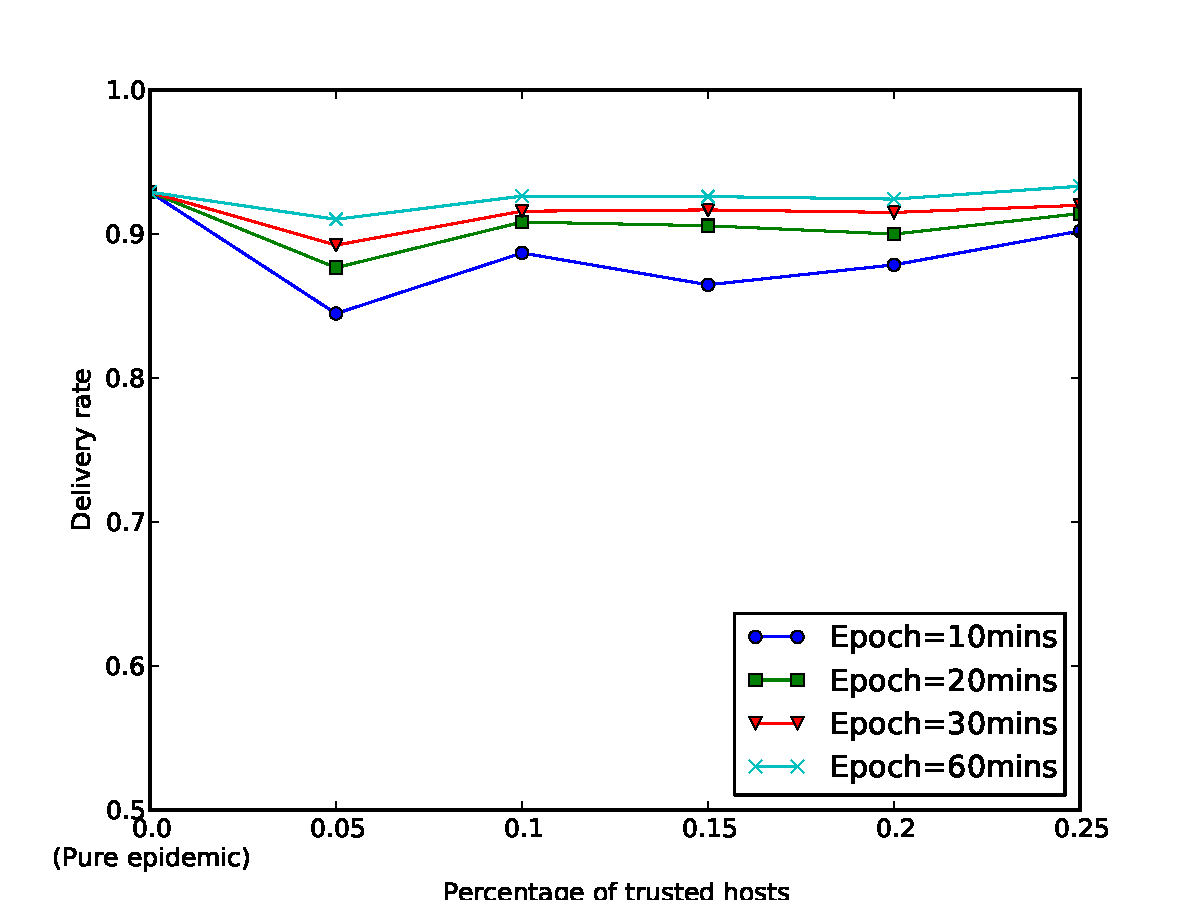
\includegraphics[width=0.49\columnwidth]{figures/normal_epoch6/delivery_rate.pdf}
\label{fig:delivery_rate_normal}
}
\hfill
\subfloat[Secure protocol]{%
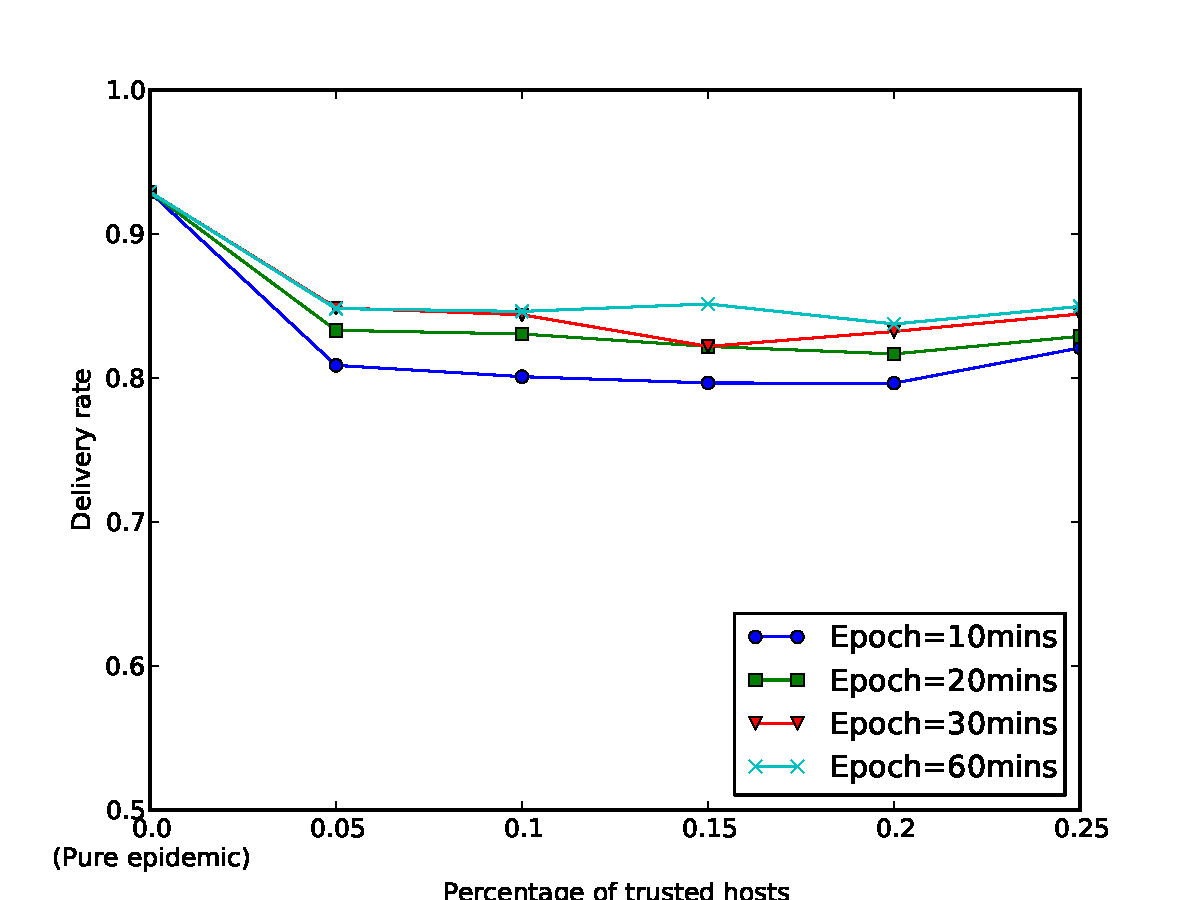
\includegraphics[width=0.49\columnwidth]{figures/secure_epoch6/delivery_rate.pdf}
\label{fig:delivery_rate_secure}
}

\caption{{\bf Overall packet delivery rate.} 
Delivery rate of pure epidemic routing: 92.91\%.  
Ephemeral ID is valid for 6 epochs. 
About 5\% drop is observed in secure protocol.
}
\label{fig:delivery_rate}
\end{figure}



% delivery rate retails
\begin{figure}[h!]
\center
\subfloat[Insecure protocol. In-group to In-group.]{%
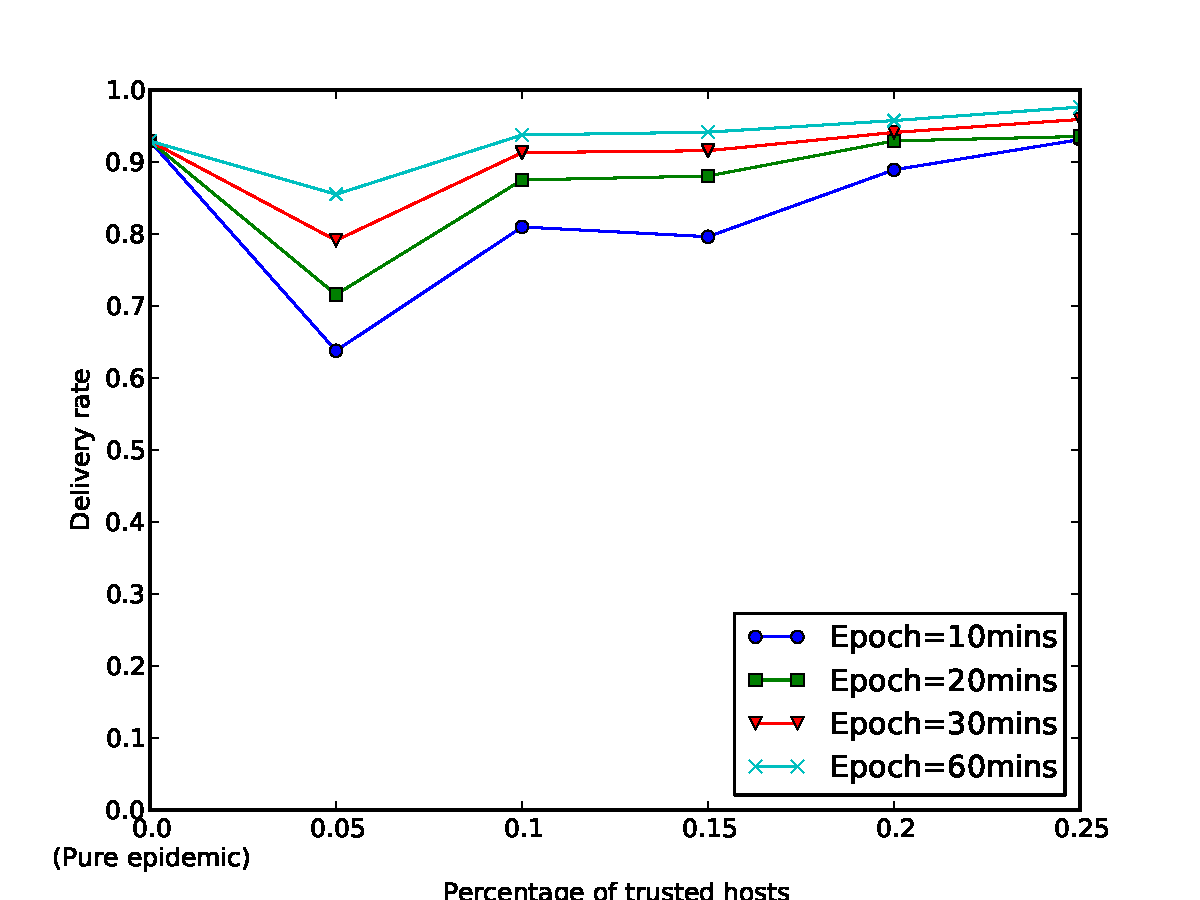
\includegraphics[width=0.33\columnwidth]{figures/normal_epoch6/delivery_rate_t_to_t.pdf}
\label{fig:delivery_rate_3_t_to_t}
}
\subfloat[Secure protocol. In-group to In-group.]{%
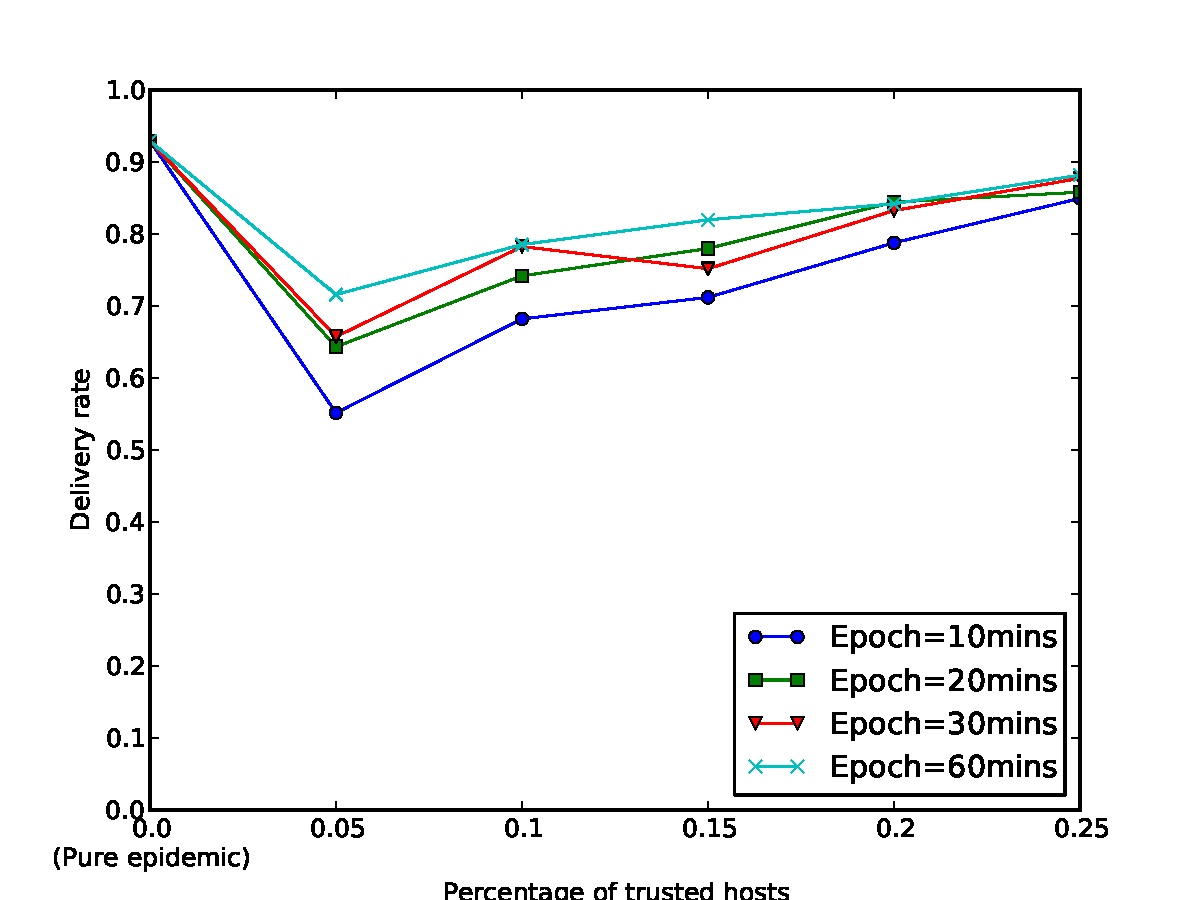
\includegraphics[width=0.33\columnwidth]{figures/secure_epoch6/delivery_rate_t_to_t.pdf}
\label{fig:delivery_rate_6_t_to_t}
}
\hfill

\subfloat[Insecure protocol. In-group to Out-of-group.]{%
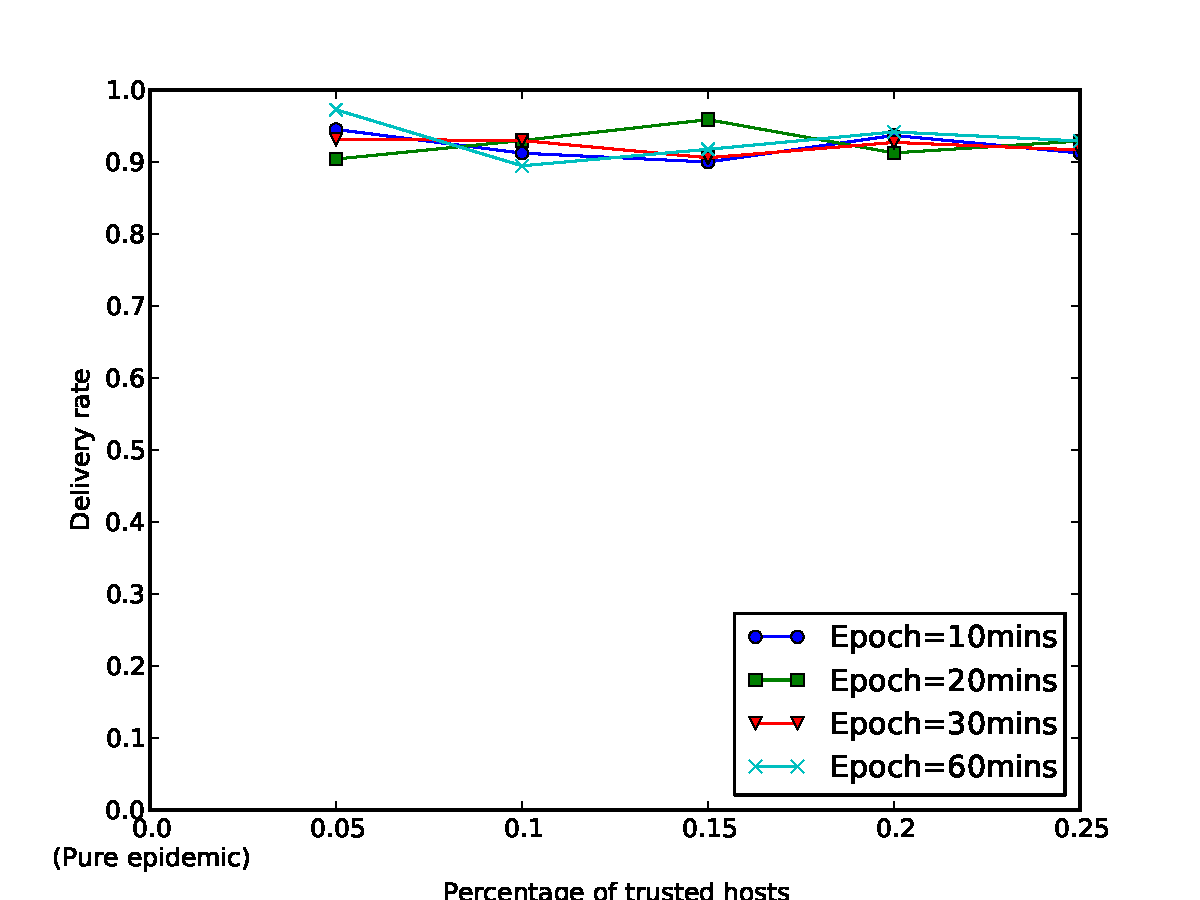
\includegraphics[width=0.33\columnwidth]{figures/normal_epoch6/delivery_rate_t_to_ut.pdf}
\label{fig:delivery_rate_3_t_to_ut}
}
\subfloat[Secure protocol. In-group to Out-of-group. ]{%
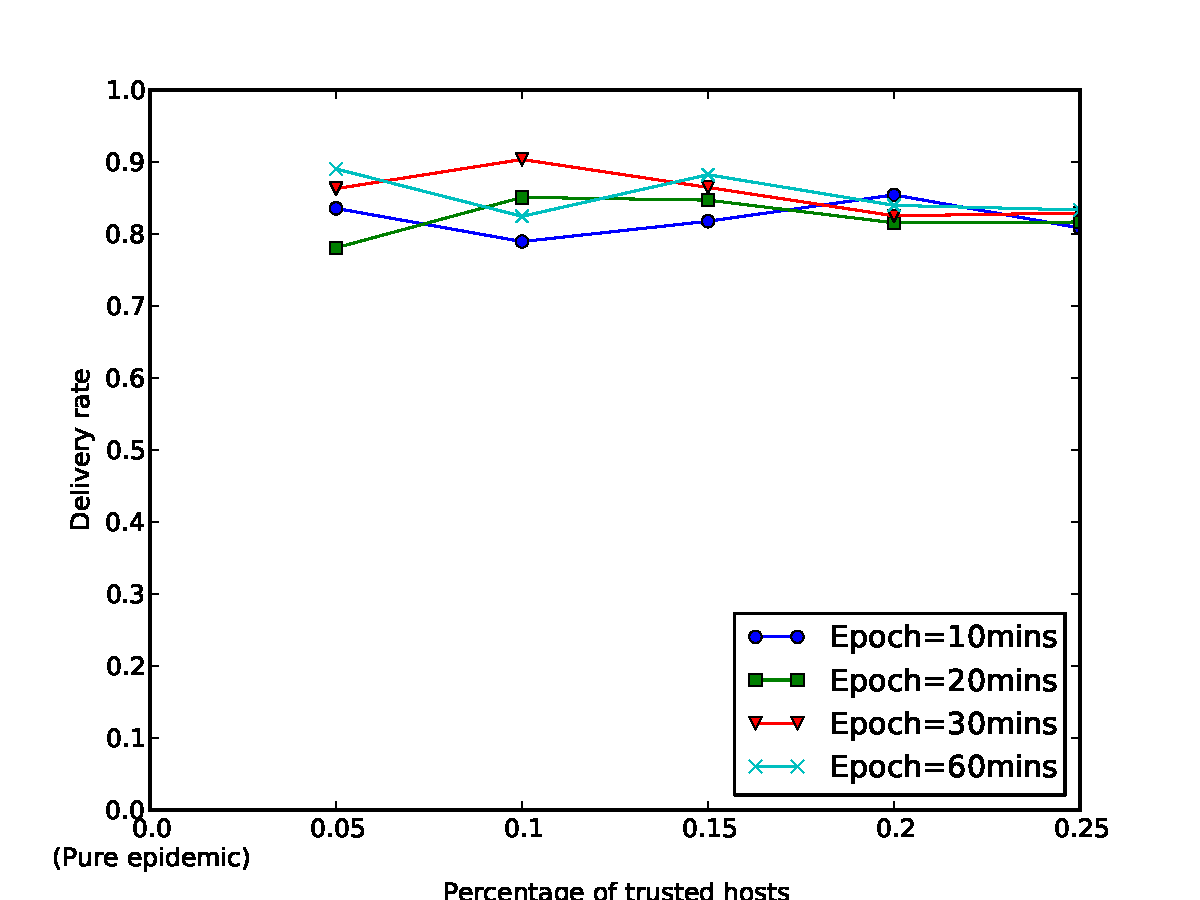
\includegraphics[width=0.33\columnwidth]{figures/secure_epoch6/delivery_rate_t_to_ut.pdf}
\label{fig:delivery_rate_6_t_to_ut}
}
\hfill

\subfloat[Insecure protocol. Out-of-group to In-group.]{%
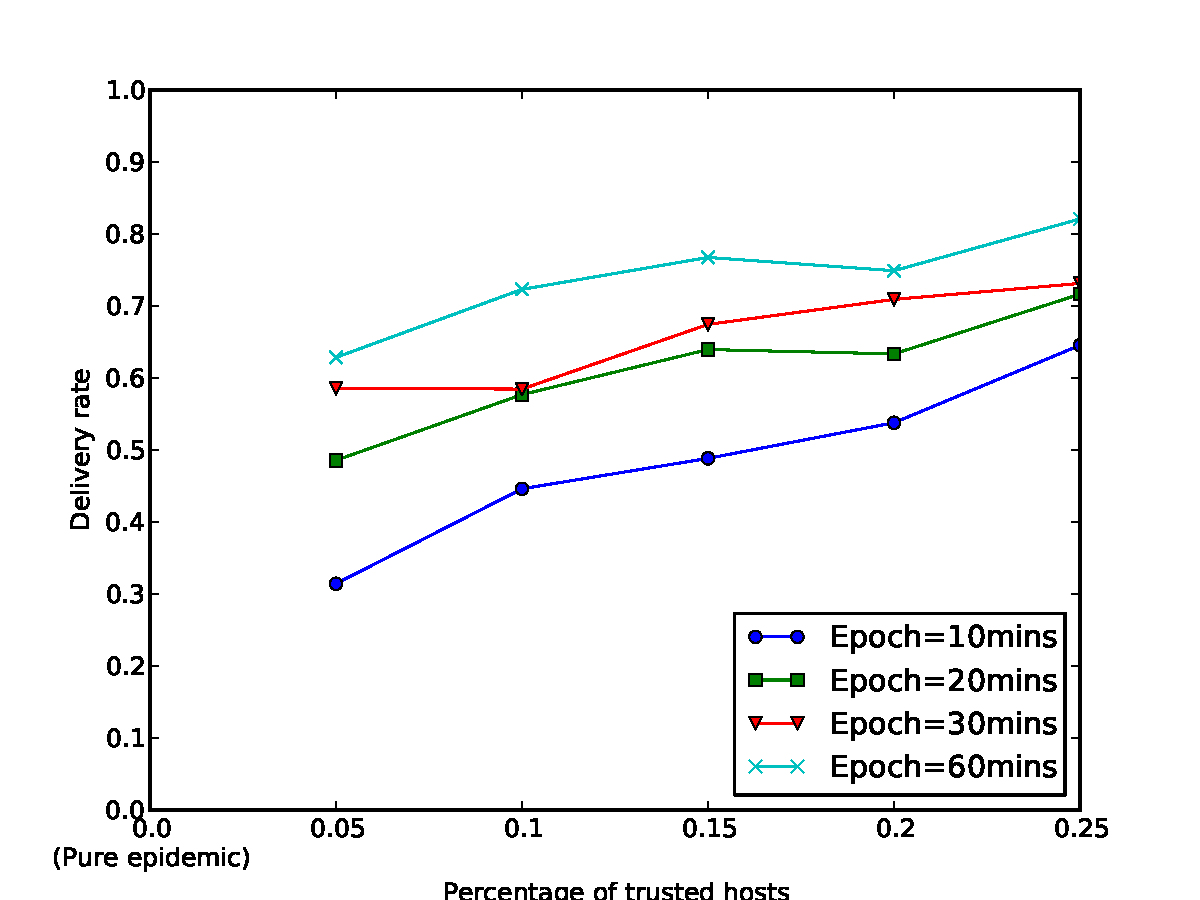
\includegraphics[width=0.33\columnwidth]{figures/normal_epoch6/delivery_rate_ut_to_t.pdf}
\label{fig:delivery_rate_3_ut_to_t}
}
\subfloat[Secure protocol. Out-of-group to In-group.]{%
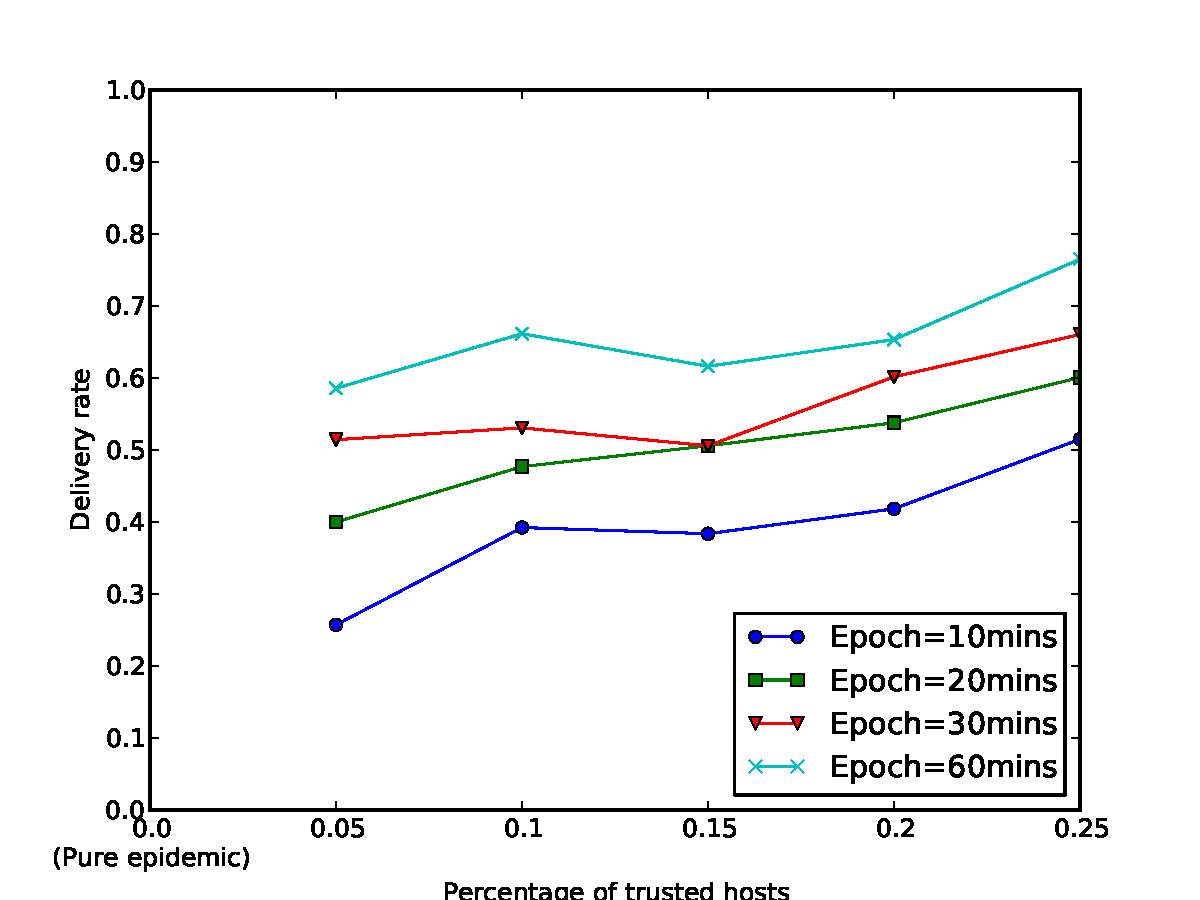
\includegraphics[width=0.33\columnwidth]{figures/secure_epoch6/delivery_rate_ut_to_t.pdf}
\label{fig:delivery_rate_6_ut_to_t}
}
\hfill

\subfloat[Insecure protocol. Out-of-group to Out-of-group.]{%
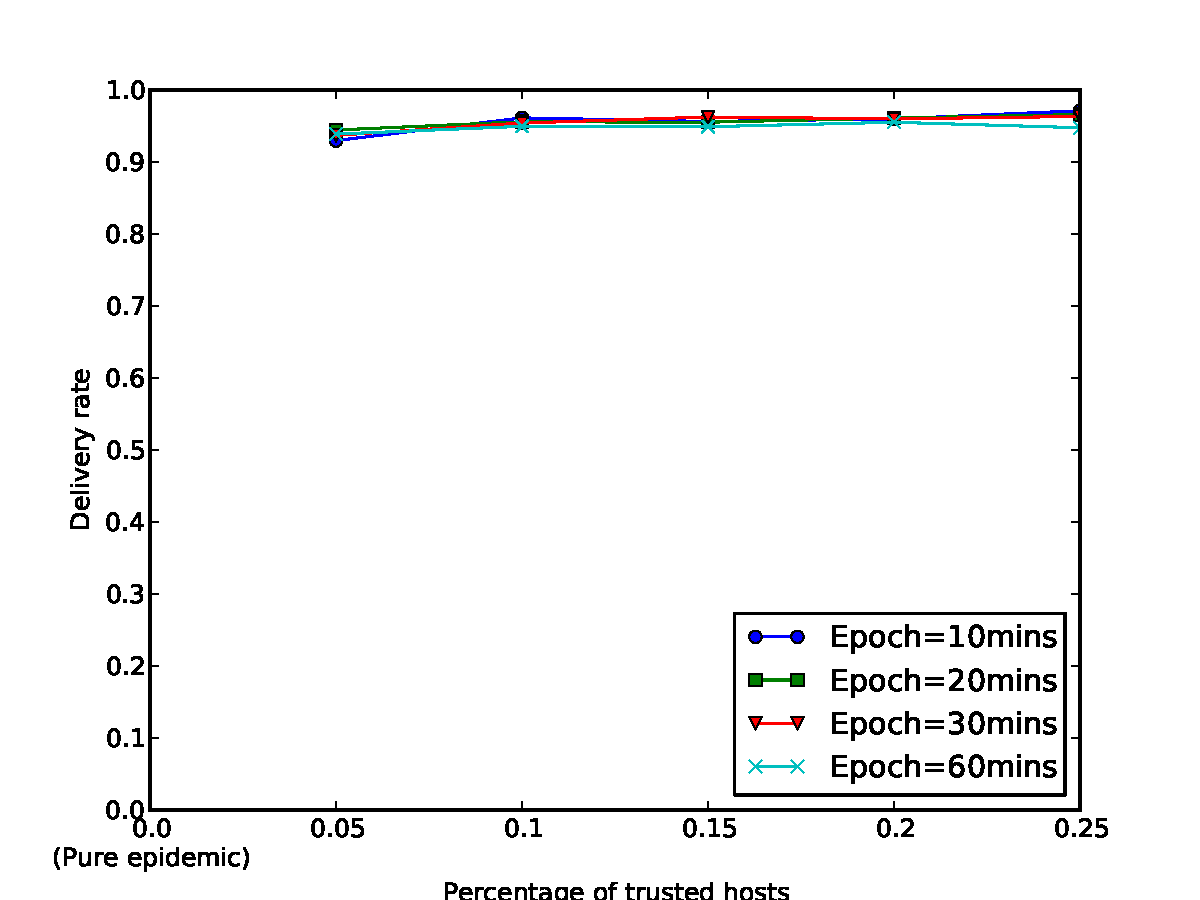
\includegraphics[width=0.33\columnwidth]{figures/normal_epoch6/delivery_rate_ut_to_ut.pdf}
\label{fig:delivery_rate_3_ut_to_ut}
}
\subfloat[Secure protocol. Out-group to Out-group.]{%
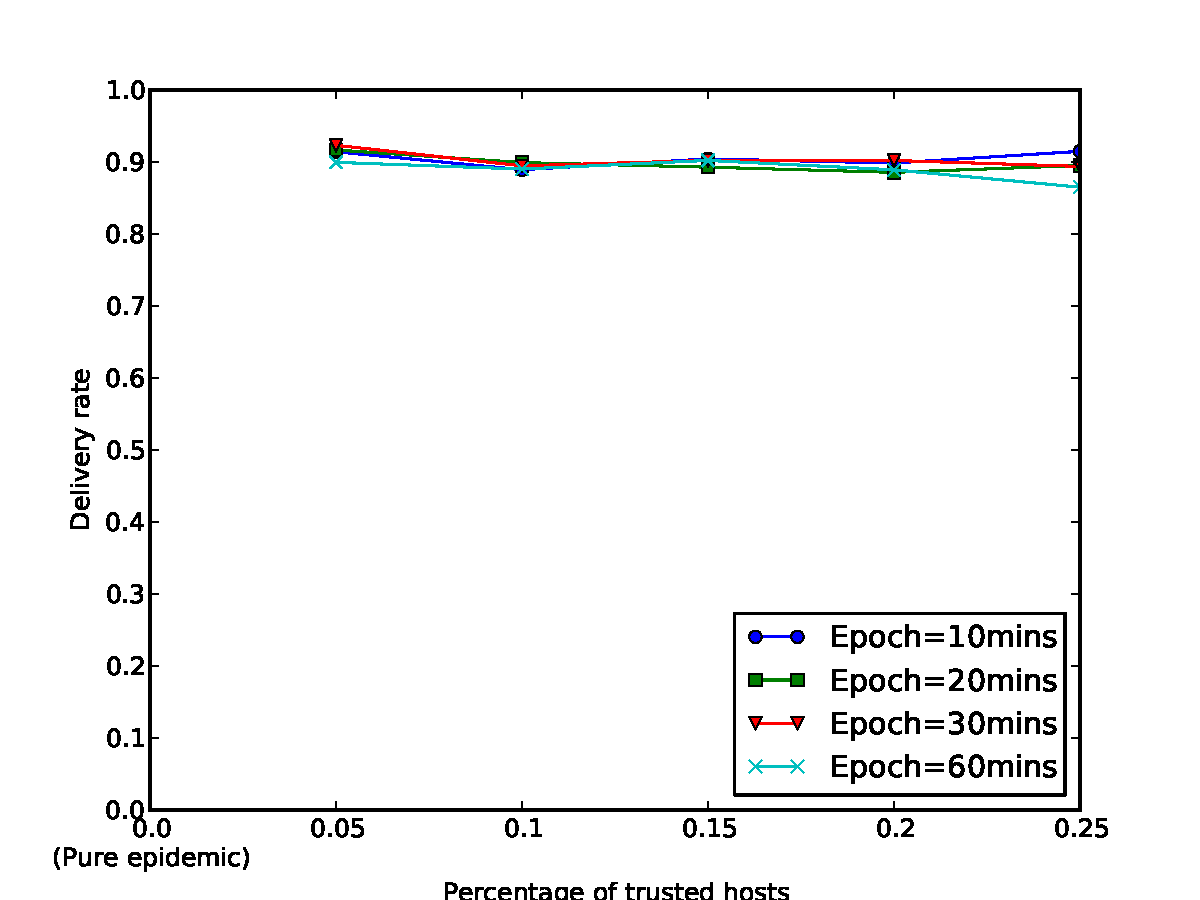
\includegraphics[width=0.33\columnwidth]{figures/secure_epoch6/delivery_rate_ut_to_ut.pdf}
\label{fig:delivery_rate_6_ut_to_ut}
}

\caption{{\bf Detailed packet delivery rate.} 
Delivery rate of `In-group' to `In-group' is decreased significantly in secure protocol. 
}
\label{fig:delivery_rate}
\end{figure}





% delivery latency
\begin{figure}[h!]
\center
\subfloat[Insecure protocol.]{%
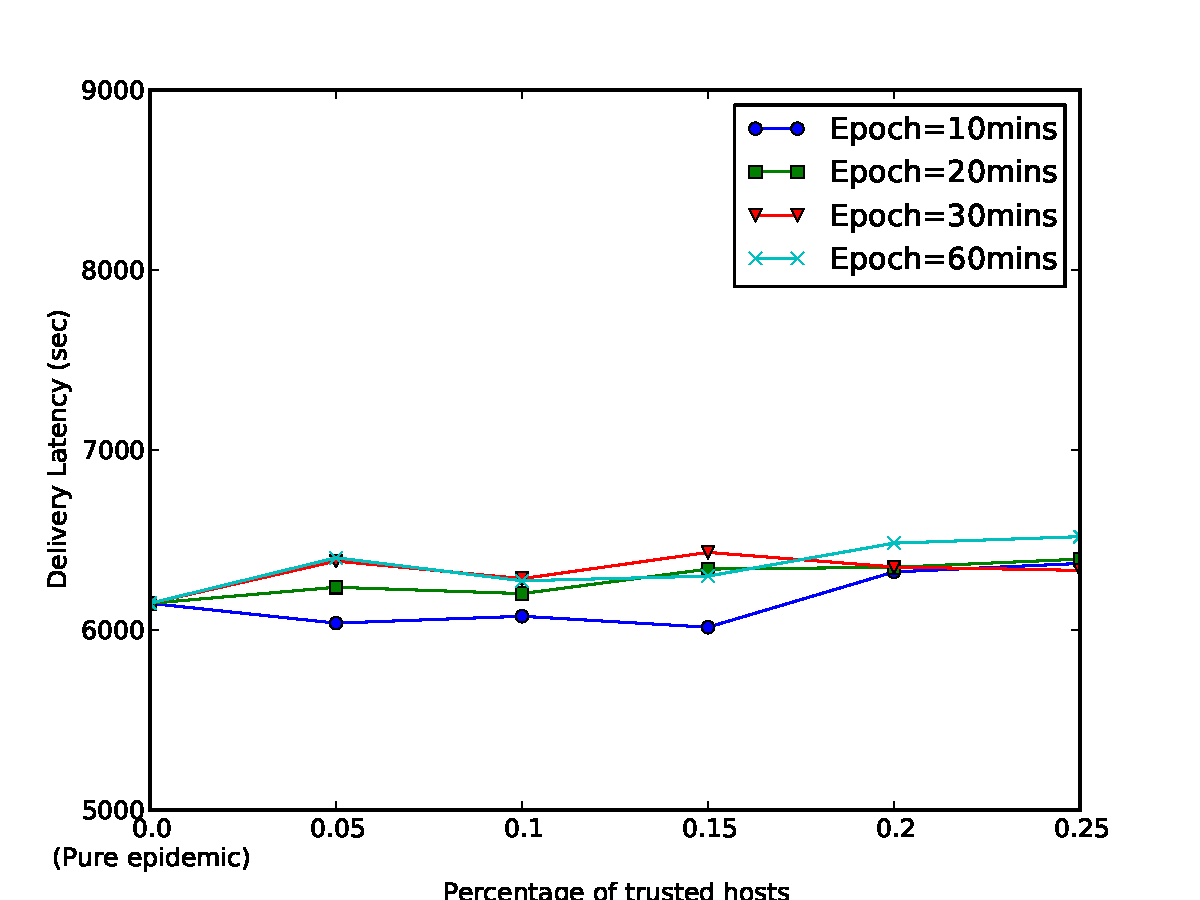
\includegraphics[width=0.49\columnwidth]{figures/normal_epoch6/delivery_latency.pdf}
\label{fig:delivery_latency_3_overall}
}
\hfill
\subfloat[Secure protocol.]{%
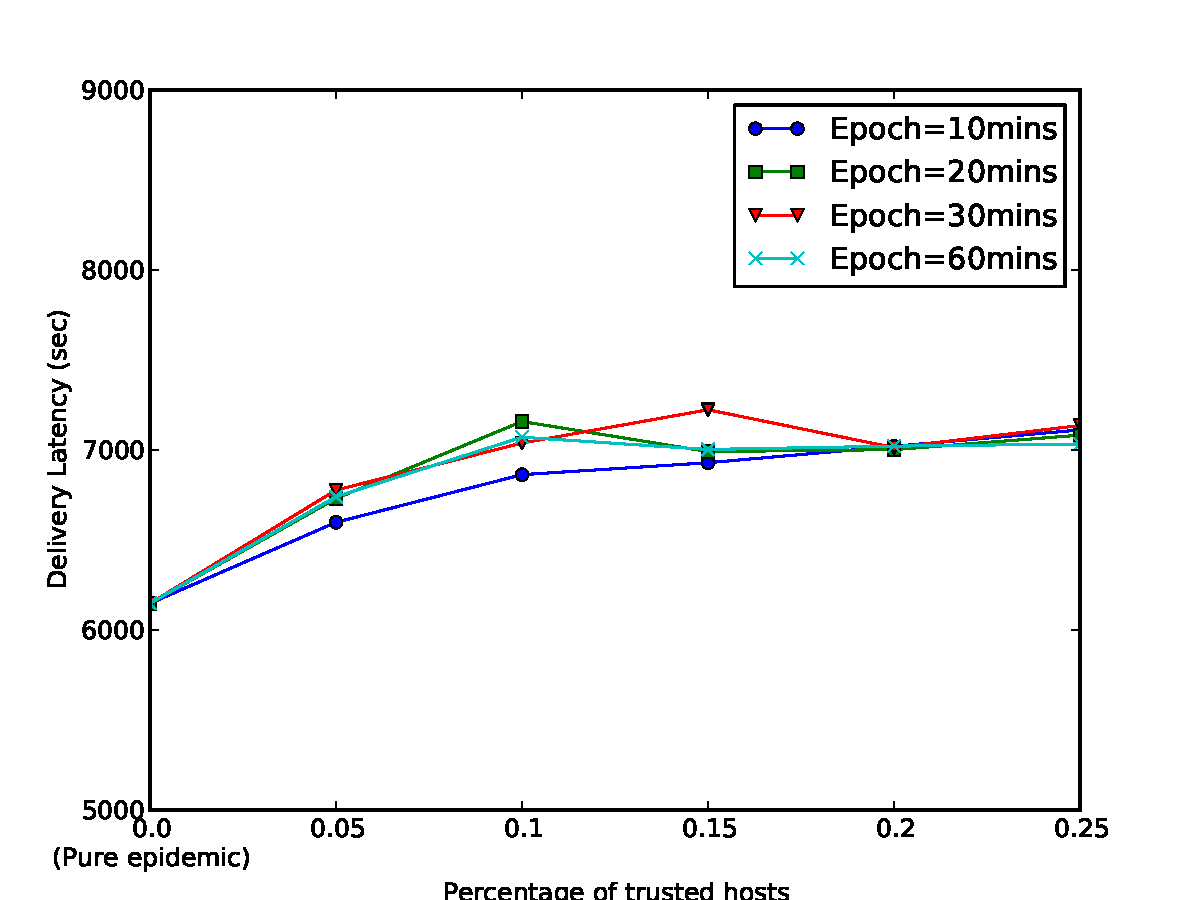
\includegraphics[width=0.49\columnwidth]{figures/secure_epoch6/delivery_latency.pdf}
\label{fig:delivery_latency_6_overall}
}

\caption{{\bf Overall packet delivery latency.}
}
\label{fig:delivery_latency_overall}
\end{figure}




% hop count
\begin{figure}[h!]
\center
\subfloat[Insecure protocol.]{%
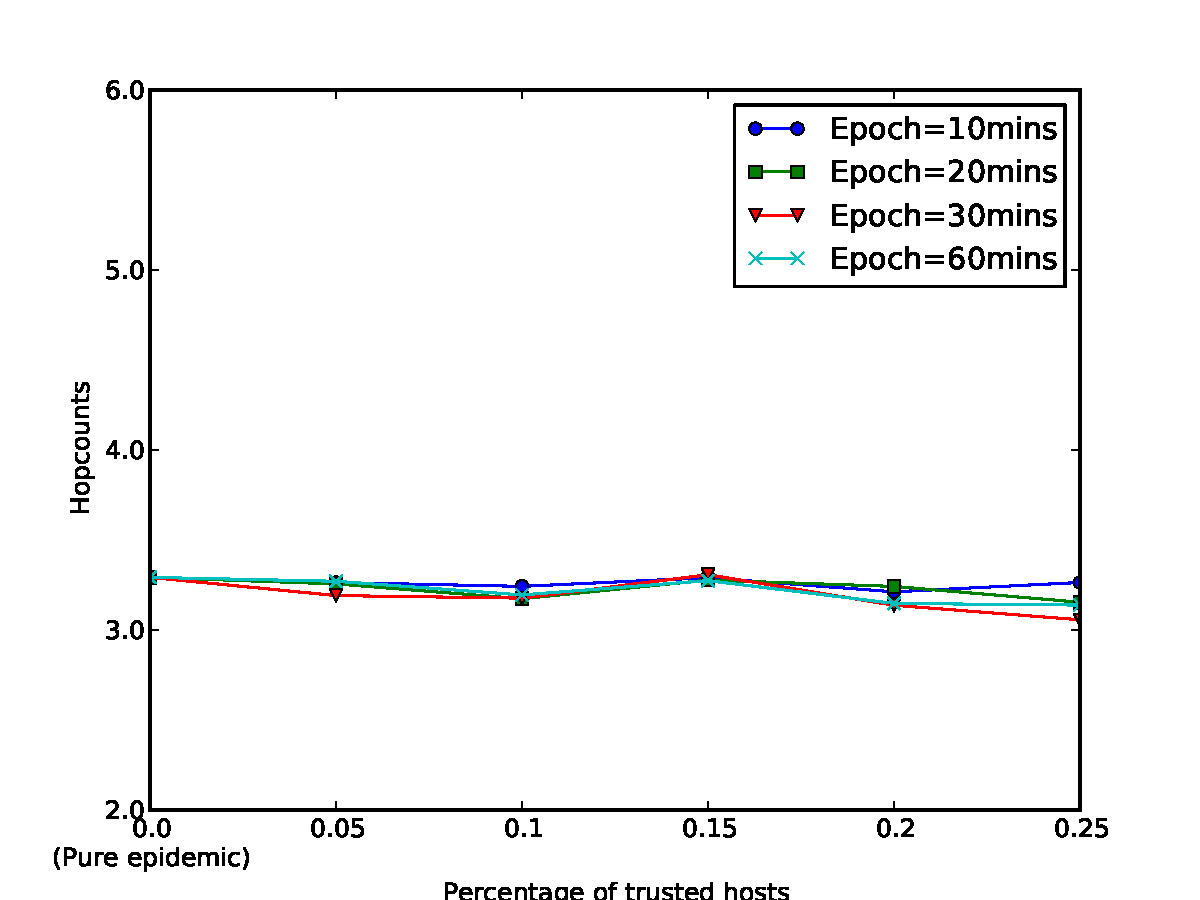
\includegraphics[width=0.49\columnwidth]{figures/normal_epoch6/hopcount.pdf}
\label{fig:delivery_hopcount_3_overall}
}
\hfill
\subfloat[Secure protocol.]{%
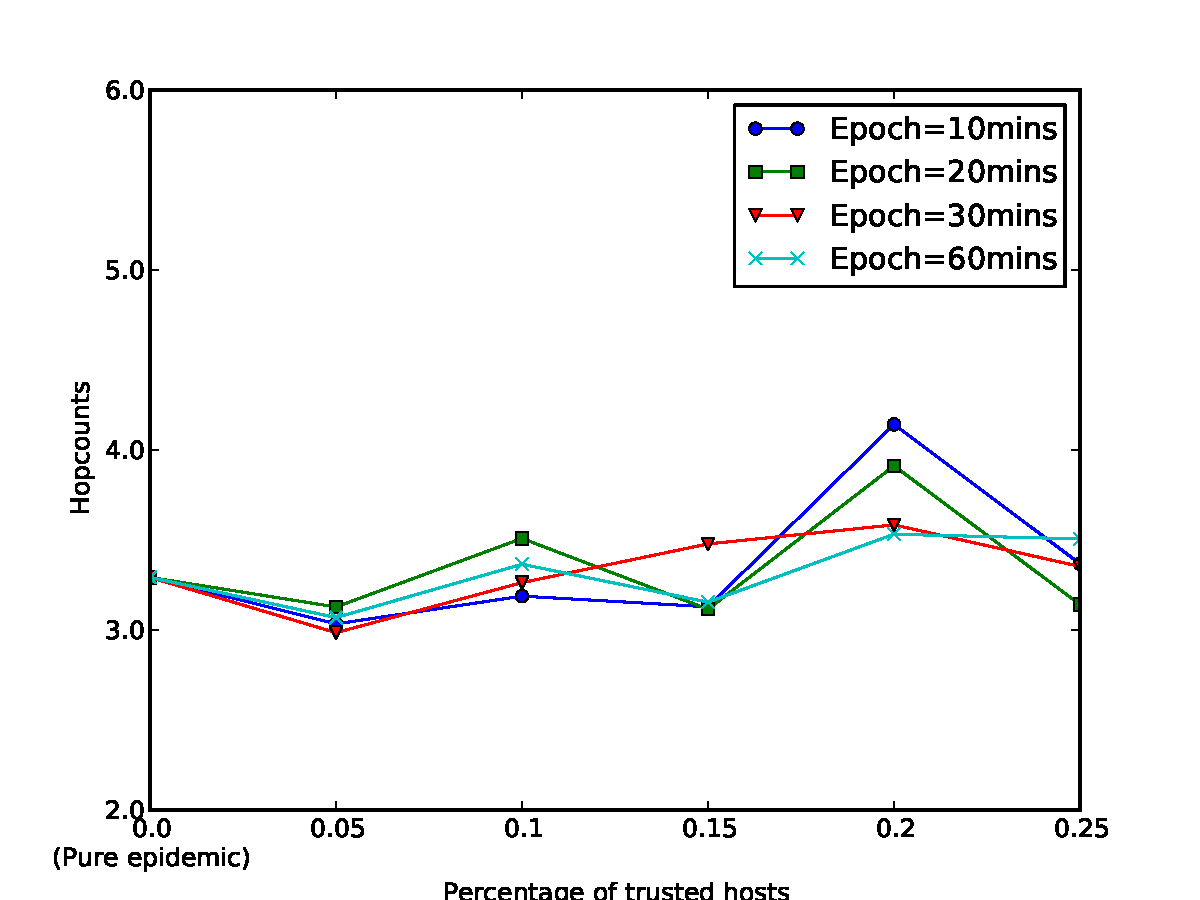
\includegraphics[width=0.49\columnwidth]{figures/secure_epoch6/hopcount.pdf}
\label{fig:delivery_hopcount_6_overall}
}

\caption{{\bf Overall packet delivery hop count.}
}
\label{fig:delivery_hopcount_overall}
\end{figure}





% packet drop classification
\begin{figure}[h!]
\center
\subfloat[Insecure protocol. Percentage of trusted nodes = 15\%.]{%
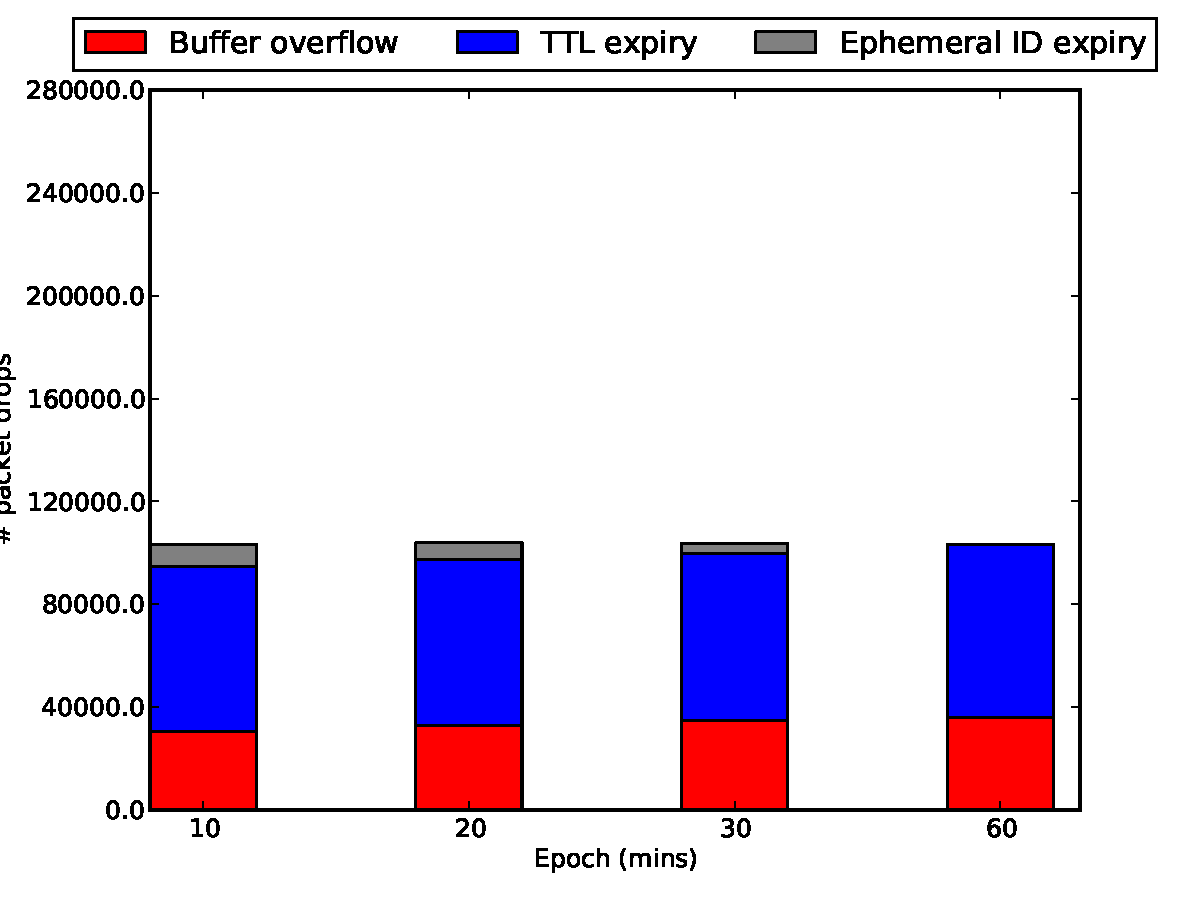
\includegraphics[width=0.49\columnwidth]{figures/normal_epoch6/drop_classification_over_epoch.pdf}
\label{fig:drop_classification_epoch_3}
}
%\hfill
\subfloat[Secure protocol. Percentage of trusted nodes = 15\%.]{%
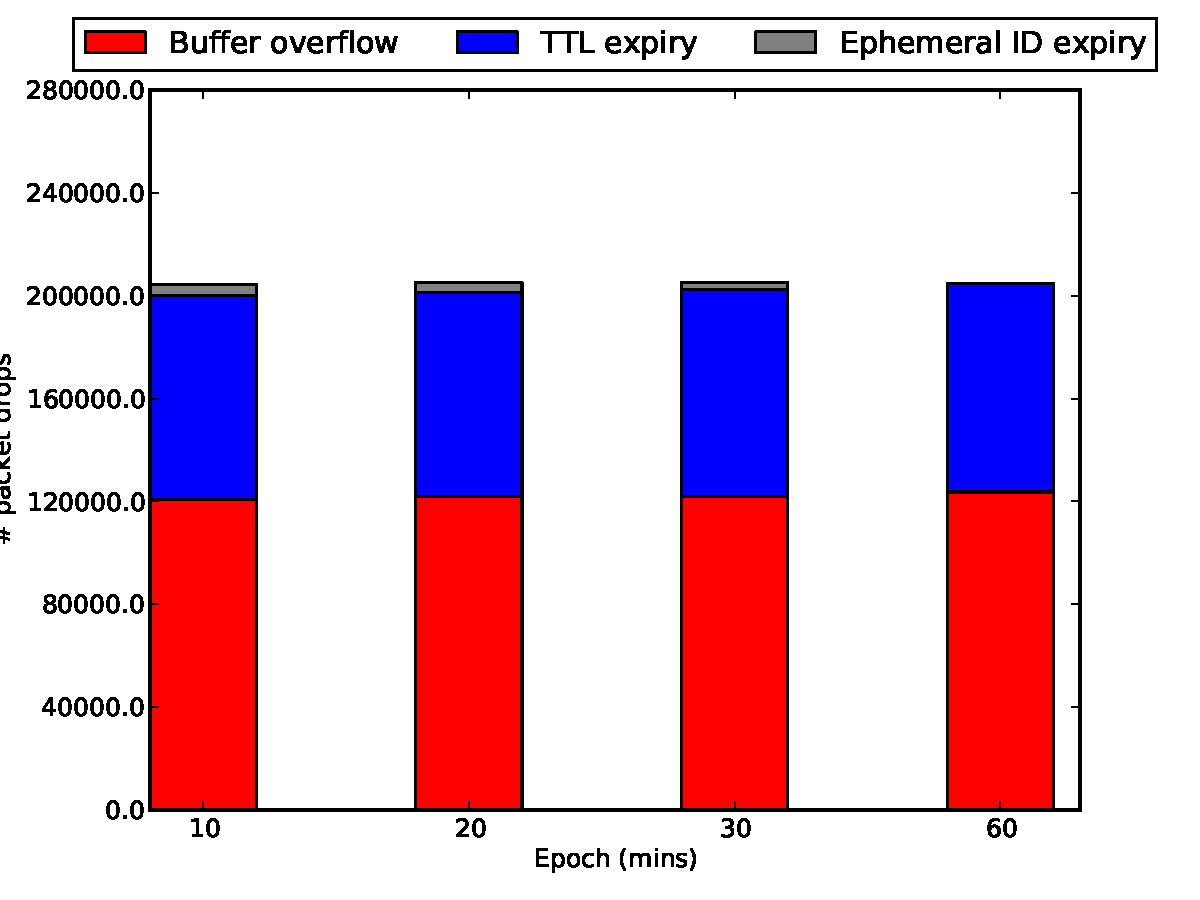
\includegraphics[width=0.49\columnwidth]{figures/secure_epoch6/drop_classification_over_epoch.pdf}
\label{fig:drop_classification_epoch_6}
}

\hfill
\subfloat[Insecure protocol. Epoch = 30 mins.]{%
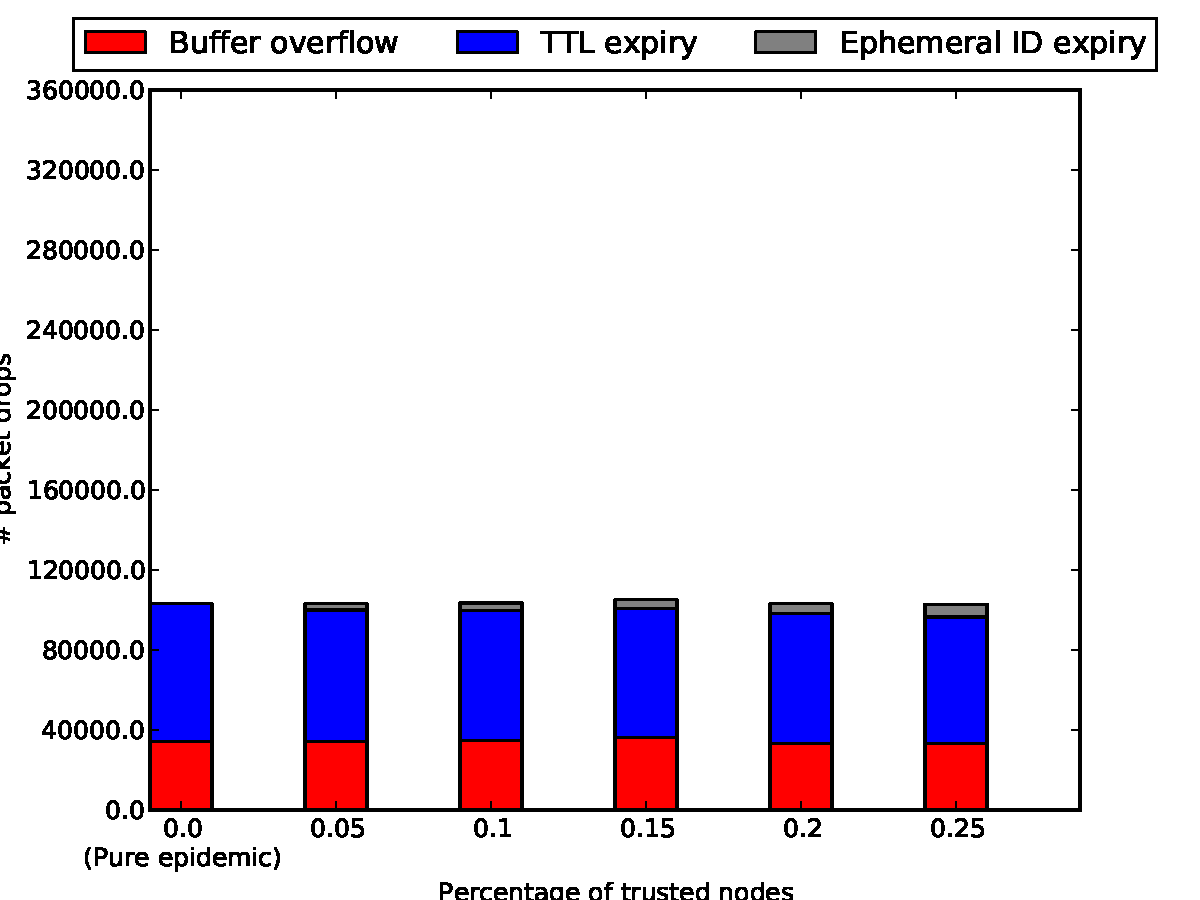
\includegraphics[width=0.49\columnwidth]{figures/normal_epoch6/drop_classification_over_percentage.pdf}
\label{fig:drop_classification_percentage_3}
}
\subfloat[Secure protocol. Epoch = 30 mins.]{%
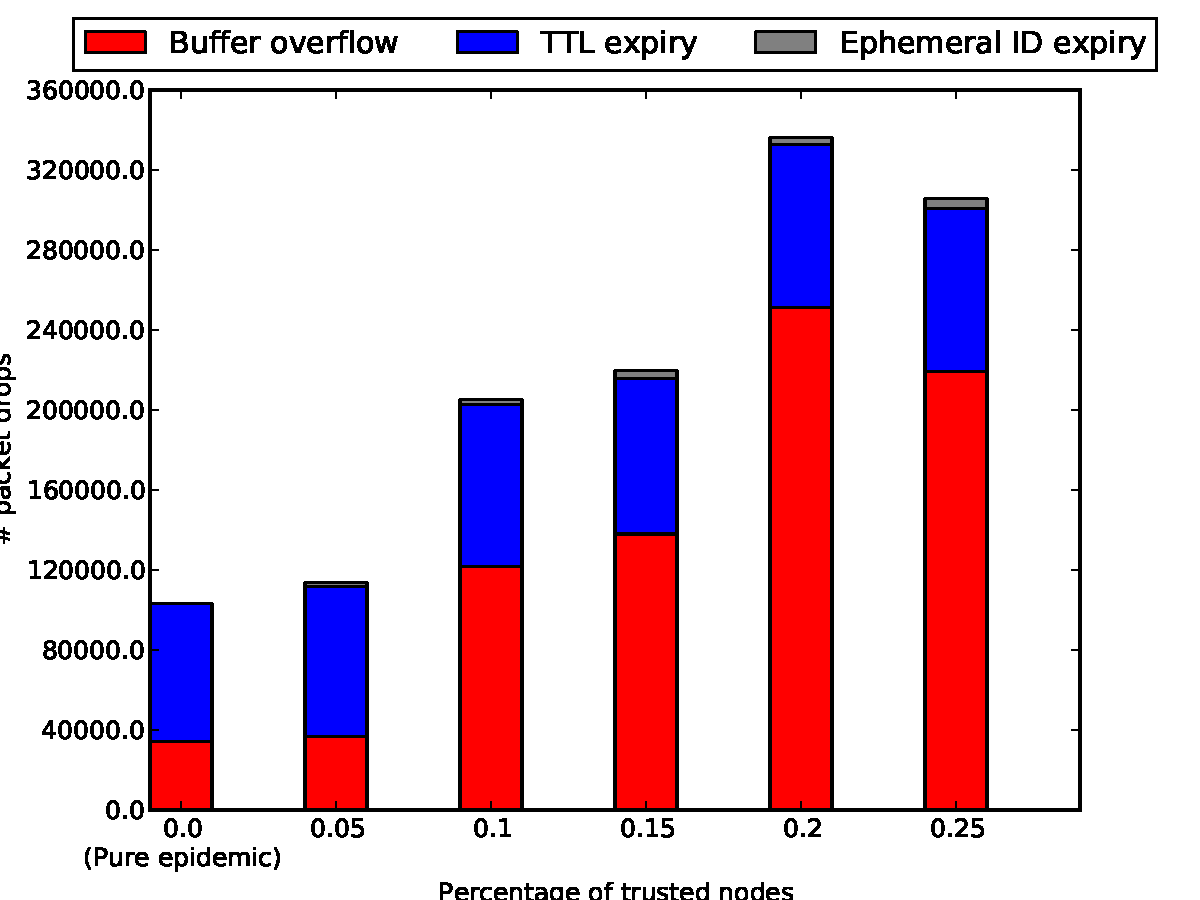
\includegraphics[width=0.49\columnwidth]{figures/secure_epoch6/drop_classification_over_percentage.pdf}
\label{fig:drop_classification_percentage_6}
}

\caption{{\bf Packet drop classification.}
New packet ID assignment in secure protocol results in more packet relays and packet drops. 
}
\label{fig:drop_classification}
\end{figure}





\end{document}







